\documentclass[a4paper,twocolumn]{article}

\usepackage[utf8]{inputenc}
\usepackage[croatian]{babel}

\makeatletter
\renewcommand\thesection{\@arabic\c@section.}
\renewcommand\thesubsection{\thesection\@arabic\c@subsection.}
\renewcommand\thesubsubsection{\thesubsection\@arabic\c@subsubsection.}
\renewcommand\theequation{\@arabic\c@equation}
\renewcommand\thefigure{\@arabic\c@figure.}
\renewcommand\thetable{\@arabic\c@table.}
\makeatother

\usepackage{algorithm}
\usepackage{algpseudocode}
\usepackage{graphicx}
\usepackage{amssymb}
\usepackage{amsmath}
\usepackage{lmodern}
\usepackage[T1]{fontenc}

\begin{document}

\title{Generator pametnih \v{s}ifri}
\author{Viktor Braut, Matija Osre\v{c}ki i Dino Suli\'c}
\maketitle

\section*{Sa\v{z}etak}

Za ve\'cinu korisnika sigurnost na ra\v{c}unalnim sustavima bazira se na
kvalitetnoj \v{s}ifri. Ovaj rad predstavlja pristup generiranju kvalitetnih
\v{s}ifri na temelju lako\'ce utipkvanja istih. Za analizu lako\'ce utipkavanja
nau\v{c}ili smo neuronsku mre\v{z}u da regresijom ocjeni lako\'cu utipkavanja
nizova znakova fiksne duljine (engl., \emph{n-gram}), u na\v{s}em slu\v{c}aju
veli\v{c}ine 3. Optimalne parametre neuronske mre\v{z}e odredili smo unakrsnom
validacijom nad skupom od oko 440 podnizova koriste\'ci 4 preklopa. Iako
rezultati jako variraju, u kona\v{c}nici smo dobili dovoljno dobre rezultate za
izradu generatora. Generator koristi jednostavnu tehniku gdje kre\'ce s
slu\v{c}ajnom odabranom kratkom \v{s}ifrom dobre kvalitete i svaki sljede\'ci znak bira
stohati\v{c}ki na temelju kvalitete novodobivenog zadnjeg podniza.

\section{Uvod}

Sigurnost privatnosti na ra\v{c}unalnim sustavima danas je bitna vi\v{s}e nego
ikada. Za ve\'cinu korisnika to zna\v{c}i jednu stvar -- kvalitetna \v{s}ifra.
I dok sustavi poput GMail-a ugra\dj uju metode dodatne verifikacije korisnika
putem tokena generiranih primjerice mobilnim ure\dj ajem te postoje
rje\v{s}enja sigurnosti uporabom kriptografskih metoda javnih i privatnih
klju\v{c}eva (SSH, GPG, itd.), za ve\'cinu web servisa, operacijskih sustava i
ostalih oblika programske potpore kvalitetna \v{s}ifra je najzastupljenije
rje\v{s}enje. 

Vi\v{s}e je svojstava kvalitetne \v{s}ifre. Najbitnije svojstvo je sigurnost --
mora biti dovoljne duljine, sadr\v{z}avati dovoljno razli\v{c}itih vrsta
znakova (mala i velika slova, brojevi i ostali znakovi) koji bi trebali biti
slu\v{c}ajno raspore\dj eni, kako pojedini dijelovi \v{s}ifre ne bi bile
konkretne rije\v{c}i. Drugo po\v{z}eljno svojstvo je da je \v{s}ifru lagano
zapamtiti. Na\v{z}alost, za ve\'cinu je to najbitnije svojstvo zbog \v{c}ega za
\v{s}ifre koriste imena svojih djevojki, velikih kantautora (jedan je Bob) i
sli\v{c}no.

U ovom radu predstavljamo ideju izbora, odnosno generiranja \v{s}ifre na
temelju lako\'ce utipkavanja iste. Prva pretpostavka je da \'ce takav na\v{c}in
zastupati sve znakove na tipkovnici u podjednakoj mjeri te da zbog slu\v{c}ajne
prirode generiranja \v{s}ifri ne\'ce do\'ci do podnizova koji se mogu na\'ci u
rje\v{c}nicima, prema tome bi trebalo biti zadovoljeno svojstvo sigurnosti.
Druga pretpostavka je da lako\'ca utipkavanja olak\v{s}ava mehani\v{c}ko
pam\'cenje i da \'ce time biti zadovoljeno drugo stvojstvo dobre \v{s}ifre,
iako mo\v{z}da tek nakon kra\'ceg perioda uvje\v{z}bavanja \v{s}ifre.

U\v{z}i aspekt ovog zadatka koji je i ujedno najte\v{z}i jest analiza lako\'ce
utipkavanja proizvoljnih nizova znakova na tipkovnici odre\dj enog rasporeda
znakova. Pristup koji smo prirodno prihvatili jest uporaba subjektivnih ocjena
skupa kra\'cih nizova u nadi da postoje nekakva statisti\v{c}ka ili geometrijska
korelacija izme\dj u transformiranih nizova znakova i na\v{s}ih subjektivnih ocjena.
Konkretno, koristili smo neuronske mre\v{z}e kako bi regresijom odredili lako\'ce
utipkvanja nizova znakova koje nismo vidjeli.

\section{Metode}

Po\v{s}to razli\v{c}iti rasporedi tipki utje\v{c}u na lako\'cu utipkavanja,
kori\v{s}ten je US raspored tipki. Tako\dj er ne koristimo znakove za koje je
potrebna tipka \texttt{shift} i podrazumijeva se da nitko ne koristi
\texttt{capslock}. Prema tome, sva slova su mala i koristi se podskup znakova.
Znakovi \texttt{\textbackslash} i \texttt{|} su na US tipkovnici na tipki koja
je ponekad iznad, a ponekad lijevo od tipke \texttt{enter}, zbog \v{c}ega
tako\dj er nisu kori\v{s}tene.

\subsection{Analiza lako\'ce tipkanja}

\subsubsection{Tehnika n-grama}

Pretpostavka koju koristimo prilikom analize lako\'ce utipkavanja proizvoljnog
teksta jest da ako uzmemo sve mogu\'ce podnizove fiksne duljine (n-grame),
lako\'ca utipkavanja tog niza znakova odgovara prosjeku ocjena lako\'ca
utipkavanja svih njegovih n-grama. Ta se pretpostavka temelji na vi\v{s}e
intuitivnih ideja. Prva je da ako su n-grami dovoljno dugi i dovoljno
kvalitetni, ono \v{s}to je trebalo utipkati prije $n$ znakova nije toliko
bitno, tj.\ toliko daleka povijest nema utjecaj na ono \v{s}to slijedi. Druga
ideja je da prilikom u\v{c}enja utipkavanja neke \v{s}ifre, korisnik \'ce
prirodno grupirati slova u manje grupe veli\v{c}ine 3 do 5, koje \'ce mo\'ci
instantno utipkati ako su kvalitetne. Time ujedno olak\v{s}avamo
ozna\v{c}avanje primjera, smanjujemo broj ulaznih kombinacija i omogu\'cujemo
u\v{c}enje neuronskim mre\v{z}om.

\subsubsection{Generiranje zna\v{c}ajki}

Za svaki znak generiramo 8 zna\v{c}ajki, koji se mogu podijeliti u tri grupe:
\begin{itemize}
        \item Koordinate trenutne tipke (2)
        \item Polarne koordinate vektora od prethodne do trenutne tipke (2)
        \item Polarne koordinate vektora od lijeve i desne tipke \texttt{alt}
            do trenutne tipke (4)
\end{itemize}
Pritom se vrijednosti svih zna\v{c}ajki normaliziraju na interval $[-1, 1]$.

Koordinate su temelj svih ovih zna\v{c}ajki. Koordinatni sustav je postavljen
sa $(0,0)$ na tipki $1$. Svaka tipka je kvadrat veli\v{c}ine $1$ sa $1$ i
udaljenost izme\dj u tipki je $0.2$. Prva koordinata je vertikalna (redak), te
horizontalna koordinata prve tipke u svakom redu je zadana nizom $[0, 0.6, 1,
1.6]$. Prema tome koordinate znaka $a$ su $(2.4, 1)$, znaka $b$ su $(3.6, 6.4)$
te za $=$ su $(0, 13.2)$. 

Polarne koordinate vektora su njegova duljina i kut, koje se trivijalno
izra\v{c}unaju uporabom Pitagorinog pou\v{c}ka i osnovne trigonometrije. Ako su
sve udaljenosti izme\dj u svih slova bliske, vjerojatno se radi o lo\v{s}em
nizu znakova jer ih vjerojatno treba upisati jednom rukom na nezgodan
na\v{c}in.

Tipke \texttt{alt} slu\v{z}e kao aproksimacija neutralne pozicije ruku tijekom
tipkanja. Naime, prsti bi prirodno trebali stajati u srednjem redu slova, nad
tipkama \texttt{asdf} i \texttt{jkl;}, ispod kojih se dva reda ni\v{z}e
pribli\v{z}no nalaze \texttt{alt} tipke. Te dvije koordinate su zapravo
izra\v{c}unate kao tipke koje bi bile direkno ispod tipki $x$ i $,$ (koordinate
$(4.8, 2.8)$ i $(4.8, 10)$). Intuicija je da ako su za jednu od ove dvije tipke
kutevi za sve znakove u n-gramu podjednaki, radi se o vertikalnom slijedu tipki
koji je primjerice nepo\v{z}eljan, dok su horizontalni slijedovi bolji.

Za n-grame veli\v{c}ine 3, koje mi koristimo, ovo sve skupa predstavlja 24
zna\v{c}ajki. Treba napomenuti da postoji 45 znakova koje koristimo, te za
n-grame duljine 3, postoji oko $10^5$ razli\v{c}itih kombinacija, od kojih je
oko $0.5\%$ pokriveno primjerima.

Osim ovog skupa zna\v{c}ajki, probali smo i pro\v{s}ireni skup sa kvadratima
svake zna\v{c}ajke. Vi\v{s}e o rezultatima kasnije.

\subsection{Stohasti\v{c}ki generator \v{s}ifri}

U ovom trenutku pretpostavljamo da imamo spremnu nau\v{c}enu neuronsku
mre\v{z}u za ocjenjivanje lako\'ce utipkavanja nekog n-grama
\texttt{ocijeni(ngram)}. 

Generator radi tako da u prvoj fazi generira n-gram dovoljne kvalitete, a zatim
u drugoj fazi gradi \v{s}ifru znak po znak do \v{z}eljene duljine. U svakom
koraku, on nasumice odabere podskup slova s kojom bi \v{s}ifra zavr\v{s}avala
n-gramom dovoljno dobre kvalitete, zatim pridaje vjerojatno odabira svakom
slovu na temelju te kvalitete te u kona\v{c}nici nasumice odabire jedno slovo
pomo\'cu diskretne slu\v{c}ajne varijable. Ukoliko u nekom trenutku nema
dovoljno slova s kojima mo\v{z}e kvalitetno nastaviti, generator bri\v{s}e
zadnje slovo i nastavlja. U tom smislu ovo nazivamo kvazi-backtracking
algoritam.

Gore navedeni algoritam ne radi pretjerano brzo i sigurno se mo\v{z}e zamijeniti
nekim oblikom evolucijskih algoritama ili nekom boljom heuristi\v{c}kom metodom,
no za potrebe prototipa i prve implementacije ove ideje radi dovoljno dobro.

\clearpage
\begin{algorithm}
\caption{Stohasti\v{c}ki generator \v{s}ifri}
\label{alg1}
\begin{algorithmic}
    \State $prag\_pocni \leftarrow 0.5$
    \State $sifra \leftarrow ``"$
    \Loop
        \State $sifra \leftarrow slucajni\_ngram()$
        \If{$ocijeni(sifra) \geq prag\_pocni$}
        \State \textbf{break}
        \EndIf
    \EndLoop\\
    \State $prag\_dalje \leftarrow 0.25$
    \While{$duljina(sifra) < zeljena\_duljina$}
        \State $promijesaj(znakovi)$
        \State $broj\_dobrih \leftarrow 0$\\
        \For{$z \in znakovi$}
            \State $ngram \leftarrow sifra[-2:] + z$
            \State $ocjena \leftarrow ocijeni(ngram)$\\
            \If{$ocjena \geq prag\_dalje$}
                \State $vjerojatnosti[z] \leftarrow ocjena + 1$
                \State $broj\_dobrih \leftarrow broj\_dobrih + 1$
            \Else
                \State $vjerojatnosti[z] \leftarrow 0$
            \EndIf
        \EndFor\\
        \State $normaliziraj(vjerojatnosti)$
        \If{$broj\_dobrih \geq 5$}
            \State $sifra \leftarrow sifra + slucajni(vjerojatnosti)$
        \ElsIf{$duljina(sifra) > 2$}
            \State $sifra \leftarrow sifra[:-1]$
        \Else
            \State \textbf{kreni ponovo}
        \EndIf
    \EndWhile
\end{algorithmic}
\end{algorithm}

\section{Rezultati}

Testiranje mreže je provedeno cross-validacijom. Od 450 primjera $75\%$ je
korišteno za učenje neuronske mreže dok je ostalih $25\%$ primjera korištena za
testiranje. Primjeri su se rotirali \v{c}etiri puta i gre\v{s}ka je usrednjena,
kako se nebi mreža uvijek učila sa istim primjerima. Kroz taj postupak
testirano je nekoliko paramatera: broj neurona u prvom sloju, broj epoha učenja
i zadovoljavajuća greška nakon koje učenje prestaje. Brojevi neurona koji su
testirani su 10, 20 i 30. Broj epoha smo ograničili na 200, 300 i 400 dok smo
za zadovoljavajuću grešku uzimali 0.001, 0.005, 0.01, 0.1 i 0.5. Za svaku
kombinaciju tih parametara izračunata je kvadratna greška (MSE). Dobiveni
podatci predočeni su grafovima na način da se vidi ovisnost greške neuronske
mreže za dva parametra te usrednjeni za tre\'ci.

\begin{figure}[htc]
    \centering
    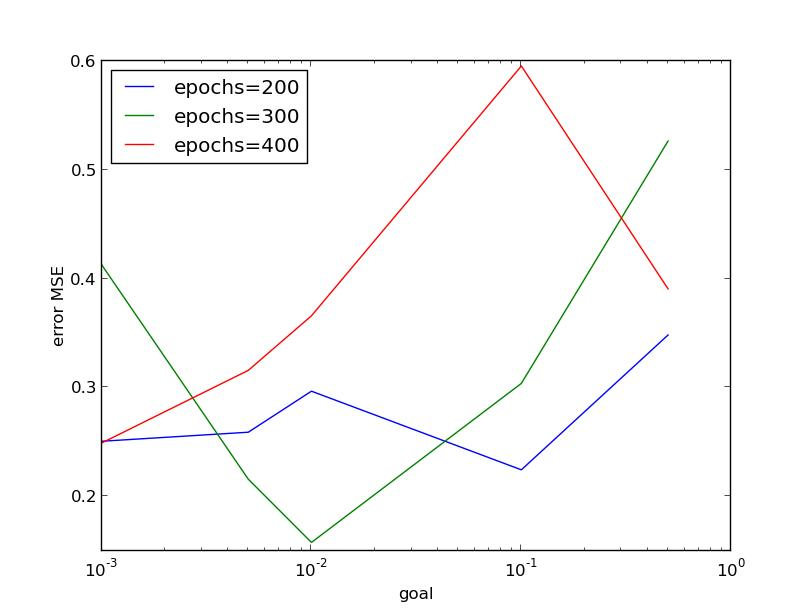
\includegraphics[scale=0.25]{epochs.jpeg}
    \caption{Odnos ciljane gre\v{s}ke i broja epoha u\v{c}enja na gre\v{s}ku}
    \label{fig:epohe}
\end{figure}

\begin{figure}[htc]
    \centering
    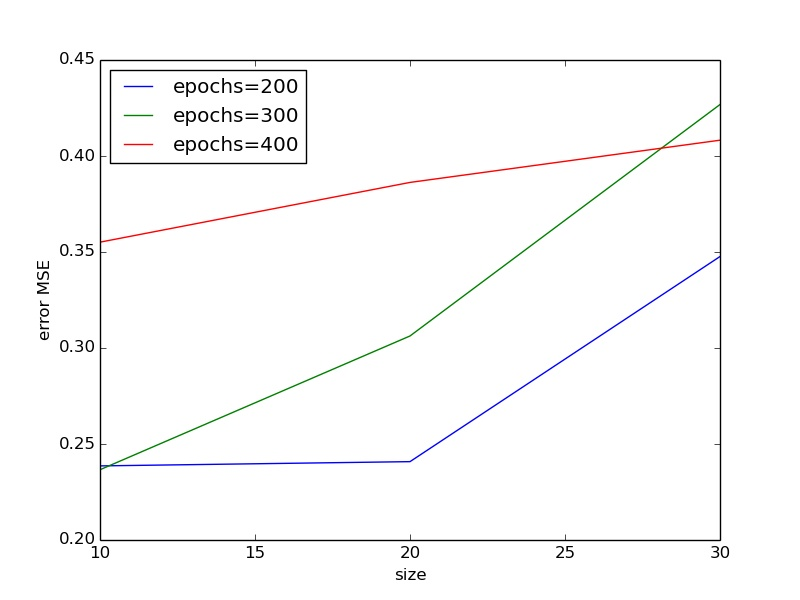
\includegraphics[scale=0.25]{goal.jpeg}
    \caption{Odnos broja neurona i broja epoha u\v{c}enja na gre\v{s}ku}
    \label{fig:greske}
\end{figure}

\begin{figure}[htc]
    \centering
    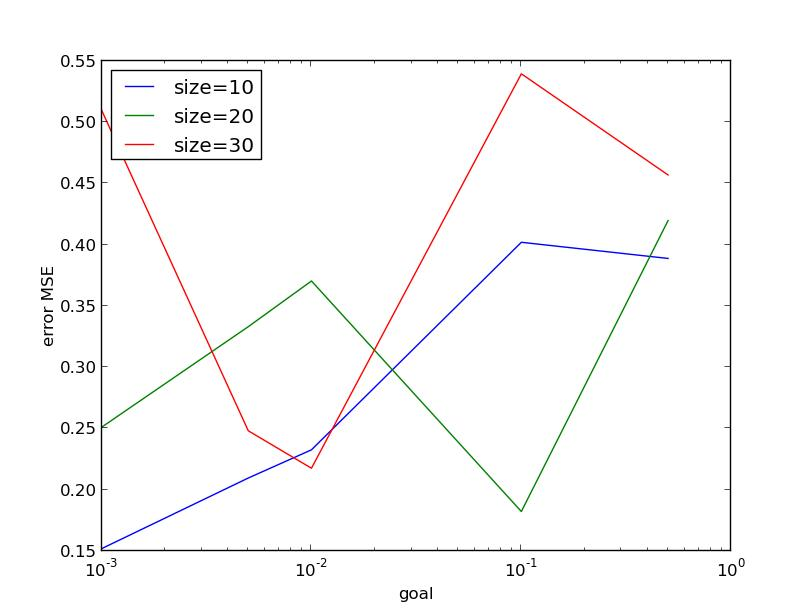
\includegraphics[scale=0.25]{size.jpeg}
    \caption{Odnos ciljane gre\v{s}ke i broja neurona na gre\v{s}ku}
    \label{fig:velicine}
\end{figure}

\section{Zaklju\v{c}ak}

Ovaj rad predstavlja prvi nama poznati pristup ideji da se kvalitetne \v{s}ifre
mogu generirati minimizacijom lako\'ce tipkanja, time osiguravaju\'ci dobar
temelj za mehani\v{c}ko pam\'cenje i sigurnost \v{s}ifre. Glavni fokus je prema
tome bila analiza lako\'ce utipkavanja proizvoljnog teksta. U tom aspektu
vjerujemo da smo postigli dovoljno dobre rezultate za na\v{s} cilj, iako
postoji mnogo mjesta za napredak.

Prvi problem je generiranje i ocjenjivanje n-grama. Vjerujemo kako je 3
apsolutno minimalna duljina i trebalo bi bolje isprobati ve\'ce duljine, ali
najvi\v{s}e do 5-6, jer nakon toga nema puno koristi. Ocjenjivanje je veoma
subjektivno, i iako je jedna ideja da je to dobro jer omogu\'cava
personalizirane generatore, upitna je statisti\v{c}ka korelacija tih ocjena i
samih n-grama. Jedna mogu\'ca ideja je napraviti program koji testira korisnika
i sam daje ocjene na temelju brzine utipkavanja. Takav program bi mogao
detektirati kada je dovoljno primjera izgenerirano i time mo\v{z}da skratiti
ionako dug postupak.

Drugi problem je kako idalno predstaviti puni skup znakova, odnosno
ukorporirati tipku \texttt{shift}. Na\v{s} prvi skup za u\v{c}enje sastojao se
od 200 n-grama duljine 4 koji su uklju\v{c}ivali sve znakove, no sa mapiranjem
shifta u posebnu zna\v{c}ajku (je li snisnut shift) za svako slovo, nismo
dobivali dobre rezultate. Mo\v{z}da je mogu\'ce maknuti to iz potprograma za
analizu i inducirati u generator, gdje bi generator odlu\v{c}ivao kada staviti
\texttt{shift} i time prilagodio ocjenu. Naravno, mo\v{z}da najbolje to
prepustiti korisniku, po\v{s}to u malo vremena mo\v{z}e odlu\v{c}iti gdje bi
\texttt{shift} odgovarao u ve\'c generiranoj \v{s}ifri.

Osim toga, mo\v{z}e se probati jo\v{s} na\v{c}ina generiranja zna\v{c}ajki kao
i druge metode strojnog u\v{c}enja.

\section*{Literatura}

Ovo smo radili isklju\v{c}ivo prema vlastitom naho\dj enju. Na internetu
je te\v{s}ko na\'ci materijale na ovu temu. Kao pomo\'c, koristili smo
isklju\v{c}ivo dokumentacije programskih biblioteka koje smo koristili
(\texttt{neurolab}, \texttt{numpy}).

\subsection*{Dodatak A: programsko ostvarenje}

Za izradu svih elemenata ovog rada kori\v{s}ten je programski jezik
\texttt{python}. Kako bi sve radilo, potrebno je instalirati pakete
\texttt{numpy} i \texttt{neurolab}.

Glavni program generatora je napisan kao samostalna skripta, ostali moduli se
mogu uvesti u recimo \texttt{ipython} i koristiti tako. Generator kao prvi
argument prima datoteku s postavkama mre\v{z}e, i onda proizvoljan broj argumenata,
svaki od kojih odgovara duljini jedne generirane \v{s}ifre. Primjer:

\begin{verbatim}
$ python easypass/main.py data/conf.net 10 12 14
10: p2a'hs]i]v
12: 4f=g=7c12hit
14: bs0.m[baikpef]
\end{verbatim}

Ostali moduli su:
\begin{quote}
\begin{description}
    \item[datagen:] generiranje podataka
    \item[util:] razne pomo\'cne metode
    \item[features:] generiranje zna\v{c}ajki
    \item[nnet:] sve za neuronske mre\v{z}e
    \item[passgen:] generator \v{s}ifri
\end{description}
\end{quote}

Za detaljni opis metoda, pogledati dokumentaciju unutar koda.

\end{document}
